\documentclass[a4paper,twoside]{article}
\usepackage[T1]{fontenc}
\usepackage[bahasa]{babel}
\usepackage{graphicx}
\usepackage{graphics}
\usepackage{float}
\usepackage[cm]{fullpage}
\pagestyle{myheadings}
\usepackage{etoolbox}
\usepackage{setspace} 
\usepackage{lipsum}
\usepackage{url} 
\setlength{\headsep}{30pt}
\usepackage[inner=2cm,outer=2.5cm,top=2.5cm,bottom=2cm]{geometry} %margin
% \pagestyle{empty}

\makeatletter
\renewcommand{\@maketitle} {\begin{center} {\LARGE \textbf{ \textsc{\@title}} \par} \bigskip {\large \textbf{\textsc{\@author}} }\end{center} }
\renewcommand{\thispagestyle}[1]{}
\markright{\textbf{\textsc{Laporan Perkembangan Pengerjaan Skripsi\textemdash Sem. Ganjil 2018/2019}}}

\onehalfspacing
 
\begin{document}

\title{\@judultopik}
\author{\nama \textendash \@npm} 

%ISILAH DATA BERIKUT INI:
\newcommand{\nama}{Ellena Angelica}
\newcommand{\@npm}{2015730029}
\newcommand{\tanggal}{15/11/2018} %Tanggal pembuatan dokumen
\newcommand{\@judultopik}{Kolektor Pengumuman Informatika} % Judul/topik anda
\newcommand{\kodetopik}{PAN4504}
\newcommand{\jumpemb}{1} % Jumlah pembimbing, 1 atau 2
\newcommand{\pembA}{Pascal Alfadian Nugroho}
\newcommand{\pembB}{-}
\newcommand{\semesterPertama}{45 - Ganjil 18/19} % semester pertama kali topik diambil, angka 1 dimulai dari sem Ganjil 96/97
\newcommand{\lamaSkripsi}{1} % Jumlah semester untuk mengerjakan skripsi s.d. dokumen ini dibuat
\newcommand{\kulPertama}{Skripsi 1} % Kuliah dimana topik ini diambil pertama kali
\newcommand{\tipePR}{B} % tipe progress report :
% A : dokumen pendukung untuk pengambilan ke-2 di Skripsi 1
% B : dokumen untuk reviewer pada presentasi dan review Skripsi 1
% C : dokumen pendukung untuk pengambilan ke-2 di Skripsi 2

% Dokumen hasil template ini harus dicetak bolak-balik !!!!

\maketitle

\pagenumbering{arabic}

\section{Data Skripsi} %TIDAK PERLU MENGUBAH BAGIAN INI !!!
Pembimbing utama/tunggal: {\bf \pembA}\\
Pembimbing pendamping: {\bf \pembB}\\
Kode Topik : {\bf \kodetopik}\\
Topik ini sudah dikerjakan selama : {\bf \lamaSkripsi} semester\\
Pengambilan pertama kali topik ini pada : Semester {\bf \semesterPertama} \\
Pengambilan pertama kali topik ini di kuliah : {\bf \kulPertama} \\
Tipe Laporan : {\bf \tipePR} -
\ifdefstring{\tipePR}{A}{
			Dokumen pendukung untuk {\BF pengambilan ke-2 di Skripsi 1} }
		{
		\ifdefstring{\tipePR}{B} {
				Dokumen untuk reviewer pada presentasi dan {\bf review Skripsi 1}}
			{	Dokumen pendukung untuk {\bf pengambilan ke-2 di Skripsi 2}}
		}
		
\section{Latar Belakang}
Pengumuman di jurusan Teknik Informatika UNPAR pada umumnya dilakukan lewat email. Pengumuman lewat email ini praktis karena tidak perlu menunggu email sampai ke tujuan dan dijamin sampai ke tujuan. Selain itu, konten yang disampaikan melalui email fleksibel. Konten tidak harus hanya tulisan tapi dapat ditambah dengan lampiran, dapat diubah gaya tulisannya, dan lain-lain. Namun, email kurang terorganisir dengan baik. Email yang masuk sering tercampur dengan email lain sehingga mahasiswa kesulitan mencari email yang penting. Dampaknya, pengumuman-pengumuman penting sering tidak terbaca secara tidak sengaja.

Pada skripsi ini, akan dibuat solusi masalah tadi dengan membangun suatu fitur. Fitur ini akan menangkap email-email pengumuman yang masuk ke sebuah email khusus untuk menangkap pengumuman. Pertama, email yang masuk ke email khusus akan diperiksa pengirimnya. Apabila pengirim adalah email yang terdaftar sebagai email yang berhak melakukan pengumuman, maka email tersebut adalah email pengumuman. Setelah itu, email tersebut akan dibuatkan permanent link dan disisipkan pada basis data. Lalu, mahasiswa akan menerima permanent link tersebut melalui notifikasi dari akun Line@. Line@ adalah layanan dari Line Corporation yang memudahkan pemilik bisnis atau organisasi menyampaikan pesan kepada pengikutnya melalui perangkat lunak pengirim pesan LINE.

Fitur ini akan dibangun sebagai fitur tambahan pada BlueTape, sebuah website milik jurusan teknik Informatika Unpar. Pembangunan fitur ini membutuhkan modifikasi BlueTape sehingga dapat dijalankan di Heroku dan menggunakan basis data PostgreSQL. Heroku adalah layanan yang memungkinkan pengembang membangun, menjalankan, dan mengoperasikan perangkat lunak di dalam internet. Selain itu, sistem ini membutuhkan beberapa fitur dari PHP IMAP dan layanan pengirim pesan LINE.

\section{Rumusan Masalah}
\begin{itemize}
\item Bagaimana cara memodifikasi BlueTape agar fitur kolektor pengumuman dapat diimplementasikan dengan bantuan Heroku dan PostgreSQL ?
\item Bagaimana cara mengimplementasikan kolektor pengumuman pada BlueTape ?
\end{itemize}

\section{Tujuan}
\begin{itemize}
\item Melakukan perawatan pada BlueTape agar fitur kolektor pengumuman dapat diimplementasikan dengan bantuan Heroku dan PostgreSQL
\item Mengimplementasikan fitur kolektor pengumuman pada BlueTape
\end{itemize}

\section{Detail Perkembangan Pengerjaan Skripsi}
Detail bagian pekerjaan skripsi sesuai dengan rencana kerja/laporan perkembangan terakhir :
\begin{enumerate}
	\item \textbf{Melakukan studi literatur tentang Heroku, Gmail, PHP IMAP, dan LINE}\\
	{\bf Status :} Ada sejak rencana kerja skripsi, kecuali PHP IMAP\\
	{\bf Hasil :}
	\begin{itemize}
		\item Heroku
		
		Heroku adalah \textit{platform cloud} yang memungkinkan pengembang untuk membangun, menjalankan, dan mengoperasikan perangkat lunak pada \textit{cloud}. Heroku mendukung beberapa bahasa pemrograman, meliputi : Ruby, Node.js, Java, Python, Clojure, Scala, Go, dan PHP.
		\begin{itemize}
			\item Arsitektur Heroku
		
			Arsitektur Heroku terdiri dari :
			\begin{itemize}
				\item Perangkat lunak
				
				Heroku mendefinisikan perangkat lunak sebagai gabungan dari \textit{source code} yang ditulis di dalam salah satu bahasa yang didukung Heroku (dapat berupa \textit{framework}), deskripsi dependensi yang dipakai, dan Procfile (jika diperlukan).
		
				\item Dependensi
		
				Dependensi adalah package yang diperlukan agar perangkat lunak dapat berjalan. Penulisan deskripsi dependensi yang dipakai tergantung pada bahasa yang dipakai. Untuk bahasa PHP, deskripsi dependensi dapat ditulis di dokumen composer.json.
		
				\item Procfile
		
				Procfile adalah dokumen yang digunakan untuk memberitahu Heroku bagian perangkat lunak yang dapat dijalankan. Procfile berisi daftar tipe proses dan cara menjalankan tipe proses tersebut.
		
				\item Tipe proses
		
				Tipe proses adalah titik masuk dari perangkat lunak. Ada tiga kelompok tipe proses : tipe proses \texttt{web}, tipe proses \texttt{worker} (tipe proses apapun selain \texttt{web}), dan tipe proses \texttt{singleton} (tipe proses yang bersifat sementara dan dapat berjalan terpisah). Di antara beragam tipe proses, ada dua tipe proses spesial : tipe proses \texttt{web} dan \texttt{release}. Tipe proses \texttt{web} adalah satu-satunya tipe proses yang dapat menerima arus HTTP eksternal dari router Heroku. Jika sebuah perangkat lunak melibatkan web server, pengembang harus menyatakannya sebagai proses \texttt{web}. Tipe proses \texttt{release} adalah tipe proses yang digunakan untuk menyebutkan perintah yang dijalankan selama fase release.
				Setiap tipe proses memiliki spesialisasinya sediri pada jenis pekerjaan tertentu. Misalnya, sebuah perangkat lunak memiliki dua jenis pekerja : pekerja untuk pekerjaan yang mendesak dan pekerja untuk pekerjaan yang berlangsung dengan lama. Dengan melakukan pembagian seperti itu, pekerjaan yang mendesak lebih cepat tertangani. Selain itu, penggunaan sumber daya lebih mudah dikontrol dan dikalkulasi.
				\begin{figure}[H]
					\centering  
					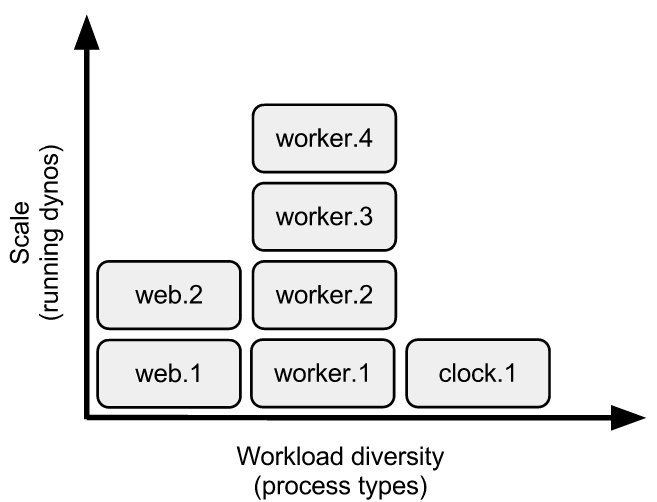
\includegraphics[scale=0.5]{Gambar/process-type-dyno-relationship.jpg}  
					\caption[Diagram hubungan antara tipe proses dan dyno]{Diagram hubungan antara tipe proses dan dyno} 
					\label{fig:process-type-dyno-relationship} 
				\end{figure}
				Tipe proses dan dyno saling berhubungan. Tipe proses adalah prototipe yang menjadi tempat dimana dyno dibentuk. Hubungan tipe proses dan dyno dapat dilihat di diagram pada Gambar~\ref{fig:process-type-dyno-relationship}. Sumbu x menyatakan tipe proses yang dipakai, sementara sumbu y menyatakan jumlah dyno yang berjalan pada tipe proses tersebut. Semakin banyak dyno pada suatu tipe proses maka konkurensi untuk pekerjaan yang ditangani tipe proses tersebut akan meningkat. Semakin banyak tipe proses maka semakin beragam beban kerja.
		
				\item Dyno
		
				Dyno adalah wadah perangkat lunak berbasis Unix yang terisolasi, tervirtualisasi, dan menyediakan lingkungan yang dibutuhkan untuk menjalankan suatu perangkat lunak. Umumnya, jika perangkat lunak di-\textit{deploy} ke Heroku untuk pertama kali, Heroku akan menjalankan satu web dyno secara otomatis. 
				Dyno dapat dikategorikan ke dalam tiga kelompok : web dyno, worker dyno, dan one-off dyno. Web dyno adalah dyno dari tipe proses "web" yang disebutkan di dalam Procfile. Web dyno adalah satu-satunya dyno yang dapat menerima arus HTTP dari router Heroku. Worker dyno adalah dyno dari tipe proses apapun selain "web" yang disebutkan di dalam Procfile. Worker dyno biasanya digunakan untuk pekerjaan di latar belakang, sistem antrian, dan pekerjaan yang memiliki jangka waktu. One-off dyno adalah dyno yang bersifat sementara yang dapat berjalan terpisah atau dengan masukan/keluaran dari terminal lokal. Dyno ini dapat digunakan untuk tugas yang bersifat administratif, seperti migrasi basis data dan sesi konsol. Dyno ini juga dapat digunakan untuk melakukan pekerjaan di latar belakang yang bersifat sesekali, seperti Heroku Scheduler.
				Heroku menyediakan beberapa tipe dyno yang berbeda. Tiap dyno memiliki sifat yang unik dan kinerja yang berbeda. Untuk semua pengguna Heroku, tersedia pilihan dyno tipe Free, Hobby, Standard, dan Performance. Ada satu tipe dyno lagi, yaitu tipe Private. Dyno tipe Private hanya tersedia di Heroku Enterpise yang diperuntukkan untuk organisasi.
		
				\item Dyno manager
		
				Dyno dikelola oleh dyno manager. Dyno manager adalah bagian dari Heroku yang bertanggungjawab untuk menjaga dyno tetap berjalan. Dyno manager melakukan pekerjaan seperti memastikan dyno didaur ulang setidaknya satu kali sehari atau setiap dyno manager mendeteksi kesalahan di dalam perangkat lunak yang berjalan. Daur ulang dyno ini berlangsung secara transparan dan otomatis secara teratur dan tercatat.
				Perangkat lunak yang menggunakan dyno tipe Free akan masuk mode sleep (tidur) jika tidak ada arus HTTP selama jangka waktu 30 menit. Ketika perangkat lunak yang tidur menerima arus HTTP, maka perangkat lunak tersebut akan terbangun. Hal ini menyebabkan perangkat lunak lebih lambat beberapa detik dari perangkat lunak yang menggunakan dyno tipe lain. Dyno tipe lain tidak memiliki mode sleep, dan akan selalu terjaga.
		
				\item Config vars
		
				Heroku memungkinkan peletakkan konfigurasi di luar source code perangkat lunak. Konfigurasi dapat diubah secara independen tanpa harus mengubah source code. Konfigurasi perangkat lunak dapat berupa informasi database, informasi kredensial, atau informasi lain yang bersifat spesifik pada perangkat lunak. Konfigurasi tersebut disimpan di dalam config vars. Config vars dapat diakses dengan cara mengakses environment variable. Cara mengakses environment variable berbeda-beda tergantung bahasa yang dipakai. Pada bahasa PHP, environment variable dapat diakses dengan getEnv().
		
				\item Add-ons
		
				Perangkat lunak biasanya memanfaatkan add-ons untuk menyediakan layanan penyokong seperti basis data, sistem antrean, layanan email, dan lainnya. Add-ons disediakan oleh Heroku atau pihak ketiga. Pengembang dapat mencari add-ons di Elements Marketplace (\url{https://elements.heroku.com/addons}). Menambah add-ons selain add-ons Heroku Postgres dan Heroku Connect membutuhkan verifikasi akun.

				\item Slug
		
				Ketika platform Heroku menerima source code perangkat lunak, heroku akan memulai proses \textit{build} (pembangunan) berdasarkan source code. Mekanisme build biasanya tergantung bahasa pemrograman yang dipakai, tapi mengikuti pola yang sama. Mekanisme build biasanya mengambil dependensi yang ditentukan, dan menciptakan aset yang diperlukan. Source code untuk perangkat lunak, dependensi yang diraih, dan hasil dari fase build digabungkan ke dalam slug. 
				Slug adalah gabungan dari source code, dependensi yang diambil, language runtime, dan hasil kompilasi atau keluaran yang dihasilkan oleh sistem build yang siap untuk dieksekusi. Slug ini adalah aspek dasar dari eksekusi perangkat lunak. Slug berisi perangkat lunak yang sudah dikompilasi, digabungkan, dan siap untuk dijalankan.
				Slug dikompilasi oleh slug compiler menggunakan buildpack. Buildpack akan mengambil perangkat lunak, dependensi, dan language runtime dan kemudian menghasilkan slug. Buildpack bersifat open source, sehingga memungkinkan pengembang memperluas Heroku ke bahasa pemrograman lain dan framework.
				Apabila ada dokumen yang tidak diperlukan untuk menjalankan perangkat lunak, pengembang dapat menambahkannya ke \texttt{.slugignore}. Dokumen ini harus dibuat di direktori root. Contoh dokumen yang mungkin ingin dimasukkan ke \texttt{.slugignore} :
				\begin{itemize}
					\item Dokumen pengolah gambar (contoh : dokumen .psd)
					\item Dokumen desain (contoh : dokumen .pdf)
					\item Data untuk pengujian
				\end{itemize}
				Ukuran slug dapat terlihat di akhir kompilasi (apabila kompilasi berhasil). Maksimum ukuran slug adalah 500 MB. Ukuran slug bervariasi berdasarkan bahasa atau framework yang digunakan, banyak dependensi yang ditammbahkan, dan faktor lain dari perangkat luank. Slug yang ukurannya lebih kecil dapat ditransfer ke dyno manager dengan lebih cepat.

				\item Buildpack
		
				Buildpack bertanggung jawab untuk mengubah source code menjadi slug, sehingga dyno dapat mengeksekusinya. Buildpack terdiri dari sekumpulan script yang ditulis dalam bahasa pemrograman yang sama dengan source code. Script tersebut akan mengambil dependensi, mengeluarkan aset atau kode yang sudah dikompilasi, dan sebagainya. Keluaran ini akan digabungkan ke dalam slug oleh slug compiler.
				Heroku akan mencari buildpack yang sesuai dan menggunakannya untuk mengompilasi perangkat lunak. Jika build sukses, buildpack yang sudah terdeteksi sesuai akan secara permanen diatur untuk push selanjutnya. Buildpack yang telah dimodifikasi dapat dipakai untuk mendukung bahasa atau framework yang tidak dapat di cakup oleh buildpack resmi.
				Biasanya buildpack yang dipakai oleh perangkat lunak hanya satu, tapi ada beberapa kasus buildpack yang dipakai tidak cukup hanya satu. Beberapa kasus tersebut adalah :
				\begin{itemize}
					\item Menjalankan buildpack untuk tiap bahasa pemrograman yang perangkat lunak gunakan. Contohnya, menjalankan JavaScript buildpack untuk aset dan buildpack Ruby untuk perangkat lunak.
					\item Menjalankan proses daemon seperti \texttt{pgbouncer} dengan perangkat lunak.
					\item Menarik dependensi sistem dengan apt.
				\end{itemize}
		
				\item Stack
		
				Stack adalah sistem operasi yang dikelola dan dipelihara oleh Heroku. Stack biasanya berlandaskan distribusi dari Linux yang ada, seperti Ubuntu. Pengembang dapat menentukan stack yang dipakai, dan buildpack akan mengubah source code menjadi paket yang dapat dieksekusi dengan stack tersebut. Saat skripsi ini dibuat, Heroku menyediakan tiga stack : Cedar-14, Heroku-16, dan Heroku-18. Cedar-14 berbasis Ubuntu 14.04 dan didukung sampai bulan April tahun 2019. Heroku-16 berbasis Ubuntu 16.04 dan didukung sampai bulan April tahun 2021. Heroku-18 berbasis Ubuntu 18.04 dan didukung sampai bulan April tahun 2023. Semua buildpack dari Heroku dapat bekerja dengan ketiga stack tersebut, namun buildpack yang merupakan hasil modifikasi belum tentu dapat bekerja dengan semua stack.
		
				\item Region
		
				Perangkat lunak di dalam Heroku dapat disebarkan ke lokasi geografis yang berbeda. Lokasi yang tersedia untuk suatu perangkat lunak tergantung pada Runtime yang dipakai oleh perangkat lunak (Common Runtime atau Private Space). Untuk perangkat lunak yang memakai Common Runtime, pengembang perlu menyebutkan region perangkat lunak saat membuat perangkat lunak. Untuk perangkat lunak yang memakai Private Space, region diatur saat membuat Private Space. Apabila pengembang tidak menyebutkan region yang dipakai, maka region akan diisi secara otomatis sebagai \texttt{us} (apabila memakai Common Runtime) atau \texttt{virginia} (apabila memakai Private Spaces).
				Region berpengaruh terhadap add-ons. Apabila add-ons tidak tersedia di region yang sama dengan perangkat lunak, maka add-ons akan gagal terpasang. Region juga dapat mempengaruhi cara kerja SSL.
		
				\item Releases
		
				Setiap ada deploy baru, perubahan di config vars, dan perubahan di daftar add-ons, Heroku akan membuat release baru dan memulai ulang perangkat lunak. Releases adalah buku besar yang mencatat setiap release tersebut. Releases ini berguna saat pengembang ingin mengembalikan perangkat lunak ke deploy lama.
		
				\item Log
		
				Log adalah catatan setiap proses yang terjadi di perangkat lunak. Heroku menggunakan Logplex untuk menyampaikan log ini. Logplex akan secara otomatis menambahkan entri log baru dari semua dyno yang berjalan di perangkat lunak, dan juga komponen lain seperti router.
		
			\end{itemize}
		
			\item Deploy perangkat lunak
		
			Heroku menggunakan Git sebagai sarana  utama untuk melakukan deploy perangkat lunak. Deploy adalah proses penyebaran perangkat lunak dari satu lingkungan ke lingkungan lain, misalnya dari lingkungan mesin pengembang perangkat lunak ke lingkungan heroku. Namun, Heroku juga menyediakan cara lain untuk melakukan deploy :
			\begin{itemize}
				\item Docker
				\item GitHub
				\item Tombol \texttt{Deploy} di dashboard Heroku
				\item WAR deployment
			\end{itemize}

			\item Basis data dan manajemen data
		
			Heroku menyediakan tiga layanan data untuk semua pelanggan :
			\begin{itemize}
				\item Heroku Postgres
			
				Heroku Postgres adalah basis data SQL yang disediakan secara langsung oleh Heroku. Heroku Postgres dapat diakses oleh bahasa apapun dengan PostgreSQL driver. Heroku secara otomatis menambahkan add-ons Heroku Postgres setiap perangkat lunak dibuat, sehingga pengembang tidak perlu menambahkannya secara manual.
			
				\item Heroku Redis
			
				Heroku Redis adalah basis data berbasis \textit{key-value store} yang bersifat \textit{in-memory}. Heroku dijalankan oleh Heroku dan dikelola sebagai add-on Heroku Redis dapat diakses oleh bahasa apapun dengan Redis driver.
			
				\item Apache Kafka
			
				Apache Kafka adalah salah satu add-on di Heroku yang disediakan oleh Kafka yang berintegrasi penuh dengan Heroku. Apache Kafka dideskripsikan Kafka dideskripsikan oleh Heroku sebagai add-on yang memungkinkan pengembang mendistribusikan perangkat lunak yang dapat menangani jutaan event dan miliaran transaksi. Kafka didesain untuk memindahkan ephemeral data yang sangat besar dengan reliabilitas yang tinggi dan toleran akan kerusakan.
			
			\end{itemize}
			Heroku juga menyediakan pilihan lain untuk pelanggan Heroku Enterprise, yaitu Heroku Connect. Selain itu, Heroku juga memungkinkan penggunaan layanan data dari pihak ketiga. Layanan data dari pihak ketiga ini tersedia sebagai add-ons.

			\item Verifikasi akun
			
			Heroku membutuhkan identitas terpercaya dan kontak dari pengguna. Heroku menganggap mempunyai informasi kartu kredit adalah cara yang paling dapat diandalkan untuk mendapatkan informasi kontak yang terverifikasi. Verifikasi akun juga membantu Heroku untuk menghindari penyalahgunaan.

			Verifikasi akun dibutuhkan untuk :
			\begin{itemize}
				\item Menggunakan lebih dari satu dyno di dalam perangkat lunak.
				\item Menambah add-on, termasuk yang gratis. Pengecualian untuk Heroku Postgres dan Heroku Connect.
				\item Mengubah domain perangkat lunak.
				\item Menerima transfer dari perangkat lunak yang memiliki sumber daya berbayar.
				\item Menambah batas standar penggunaan one-off dyno.
				\item Memiliki lebih dari 5 perangkat lunak dalam satu waktu.  Akun yang terverifikasi dapat memiliki sampai 100 perangkat lunak.
			\end{itemize}

			Cara melakukan verifikasi akun Heroku :
			\begin{itemize}
				\item Pergi ke Account Settings (\url{https://dashboard.heroku.com/account})
				\item Menekan tab Billing
				\item Menekan tombol Add Credit Card
			\end{itemize}

			Kartu kredit yang diterima oleh Heroku adalah kartu Visa, MasterCard, American Express, Discover dan JCB. Kartu debit juga diterima untuk kartu Visa, MasterCard atau JCB. Kartu lain tidak diterima. Beberapa bank mungkin mensyaratkan penahanan satu dollar oleh pelaku verifikasi sebelum kartu dapat dikonfirmasi.
		
		\end{itemize}
		
		\item Gmail		
		
		\begin{itemize}
			\item Resource
			
			\begin{itemize}
				\item Message
				
				Message merepresentasikan surat elektronik. Message hanya bisa dibuat atau dihapus. Tidak ada properti dari message yang bisa diubah selain label yang diberikan ke message.
				
				\item Label
				
				Label berfungsi sebagai sarana utama untuk mengelompokkan dan mengatur message dan thread. Label mempunyai hubungan banyak ke banyak dengan message. Artinya, satu message dapat memiliki beberapa label dan satu label dapat diberikan ke beberapa message.
				Label ada dua jenis : label sistem dan label pengguna. Contoh label sistem adalah label INBOX, TRASH, dan SPAM. Label sistem dibuat secara internal dan tidak dapat dibuat, dihapus, dan dimodifikasi. Namun, beberapa label sistem dapat diberikan ke message atau dilepaskan dari message. Label pengguna dapat ditambah, dihapus, dan dimodifikasi oleh pengguna atau perangkat lunak.
				
				\item Draft
				
				Draft merepresentasikan message yang belum dikirim. Message tidak bisa dimodifikasi setelah dibuat, tapi message yang terdapat di dalam draf dapat dimodifikasi. Mengirimkan draft secara otomatis akan menghapus draft tersebut dan membuatnya menjadi message dengan label sistem SENT.
				
				\item History
				
				History adalah riwayat modifikasi message yang diurutkan secara kronologis. History hanya menyimpan perubahan dalam jangka waktu 30 hari.
				
				\item Thread
				
				Thread adalah kumpulan message yang merepresentasikan percakapan. Thread dapat memiliki label. Thread tidak dapat dibuat, tapi dapat dihapus. Message dapat dimasukkan ke Thread.
				
				\item Setting
				
				Setting mengontrol perilaku fitur pada Gmail kepda User. Setting tersedia untuk akses POP dan IMAP, forward email, filter, vacation auto-response, send-as aliases, signatures, dan delegates.
				
			\end{itemize}
			
			\item Scope
			
			Gmail API menggunakan OAuth 2.0 untuk menangani autentikasi dan authorization. Pengembang harus menyebutkan scope yang dipakai di perangkat lunak. Scope adalah string yang mengidentifikasi resource yang ingin di akses. Scope ini digunakan bersama dengan token untuk mengamankan akses ke resource pengguna. Contoh scope :
			\begin{itemize}
				\item \url{https://www.googleapis.com/auth/gmail.readonly} : scope untuk membaca message dari Gmail
				\item \url{https://www.googleapis.com/auth/gmail.modify} : scope untuk mengubah label pada thread atau message
				\item \url{https://www.googleapis.com/auth/gmail.compose} : scope untuk mengirim message mewakili pengguna
			\end{itemize}
			
			\item Penggunaan pada umumnya
			
			\begin{itemize}
				\item Mengirim message

				\begin{enumerate}
					\item Membuat konten email
					\item Membuat string yang dikodekan berdasarkan base64url dari konten
					\item Membuat resource message dan memasukkan string tersebut ke properti \texttt{raw}
					\item Memanggil \texttt{message.send} untuk mengirim message
				\end{enumerate}

				\item Mengambil email yang diterima
			
				Mengambil email yang diterima membutuhkan ID email. Mengambil email yang diterima dapat dilakukan dengan metode \texttt{get} dari resource User.messages. Saat mengambil message, format dari respon dapat diatur. Format \texttt{FULL} mengembalikan seluruh informasi dari message. Format \texttt{MINIMAL} hanya mengembalikan metadata seperti label. Format \texttt{RAW} mengembalikan properti \texttt{raw} saja. Secara otomatis, format dari respon memakai format \texttt{FULL}.
			
				\item Perubahan di history
			
				Perubahan message direpresentasikan oleh \texttt{History objects}. Properti \texttt{start\_history\_id} memperbolehkan pengembang mengatur dari titik mana perubahan ingin dikembalikan. Beberapa perubahan dapat mempengaruhi lebih dari satu message, sehingga history yang merepresentasikan perubahan tersebut akan berisi beberapa message.
			
				\item Manajemen Label
			
				Label yang diberikan ke sebuah thread juga diberikan ke semua message di dalam thread. Jika sebuah label dihapus, label tersebut akan dihapus dari semua thread dan message yang memiliki label tersebut. Properti \texttt{messageListVisibility} digunakan untuk menentukan apakah message dengan label tersebut ada di message list. Properti \texttt{labelListVisibility} digunakan untuk menentukan apakah ada label tersebut di daftar label. Untuk mengubah label, gunakan \texttt{messages.modify} dan\texttt{threads.modify}.
			
			\end{itemize}
			
		\end{itemize}
		
		\item PHP IMAP
		
		PHP IMAP adalah layanan PHP untuk mengakses email melalui protokol IMAP.  Berikut adalah \textit{function} dasar dari imap :
		\begin{itemize}
			\item imap\_8bit : melakukan konversi 8bit string ke quoted-printable string
			\item imap\_alerts : mengembalikan semua pesan peringatan dari IMAP yang telah terjadi
			\item imap\_base64 : decode BASE64 encoded text
			\item imap\_binary : melakukan konversi 8bit string ke base64 string
			\item imap\_body : membaca message body
			\item imap\_bodystruct : membaca struktur dari bagian body tertentu dari message tertentu
			\item imap\_check : mengecek mailbox (kotak surat)
			\item imap\_close : menutup IMAP stream
			\item imap\_errors : mengembalikan semua error dari IMAP yang telah terjadi
			\item imap\_fetch\_overview : membaca informasi pada header dari message yang diberikan
			\item imap\_fetchbody : mengambil bagian tertentu dari message body
			\item imap\_fetchheader : mengembalikan header dari message
			\item imap\_fetchmime : mengambil MIME headers dari bagian tertentu dari message
			\item imap\_fetchstructure : membaca struktur dari message tertentu
			\item imap\_headerinfo : membaca header dari message
			\item imap\_open : membuka IMAP stream ke mailbox
			\item imap\_qprint : melakukan konversi dari quoted-printable string ke 8 bit string
			\item imap\_sort : mendapatkan dan menyortir message
			\item imap\_utf8 : melakukan konversi dari MIME-encoded text ke UTF-8
		\end{itemize}
		
		\item LINE
		
		Line Menyediakan Messaging API untuk membangun messaging bot. Messaging API memungkinkan data dioper antara server dari perangkat lunak bot dengan LINE Platform. Ketika pengguna Line mengirimkan pesan ke bot, sebuah webhook akan terpicu dan LINE Platform akan mengirimkan permintaan ke URL webhook bot. Server akan mengirim permintaan ke LINE Platform untuk merespon pengguna. Permintaan akan dikirimkan dalam format JSON.
		
		Pengembang dapat melakukan hal-hal berikut dengan Messaging API :
		\begin{itemize}
		\item Mengirimkan reply message
		\item Mengirimkan push message
		\item Mengirimkan berbagai jenis pesan
		\item Mendapatkan profil pengguna yang berinteraksi dengan bot
		\item Bergabung dengan percakapan grup /group chats
		\end{itemize}

		Untuk menggunakan Messaging API, pengembang memerlukan akun LINE@. Messaging API juga dapat digunakan menggunakan akun resmi /official accounts. Akun resmi mendapatkan fitur tambahan untuk pengguna enterprise.
		
		Untuk memulai membangun bot dengan Messaging API, pengembang perlu membuat channel terlebih dahulu. Channel adalah penyambung antara LINE platform dan perangkat lunak yang dibuat pengembang.
		
		Setelah membangun channel, pengembang perlu menyiapkan server untuk menjadi host dari bot. Pengembang dapat menggunakan layanan cloud platform, seperti Heroku. Setelah itu, pengembang dapat mulai mengatur bot pada console.

		Perangkat lunak bot membutuhkan channel access token untuk membuat API call dan webhook URL untuk menerima webhook payload dari LINE Platform. Channel access token adalah long-lived token (token yang tidak memiliki kadaluarsa) yang harus diatur di dalam authorization header ketika membuat API call. Pengembang dapat menerbitkan lagi channel access token kapanpun melalui console. Untuk menerbitkan channel access token, klik Issue pada "Channel settings" di halaman console. Sedangkan webhook URL adalah titik akhir dari server perangkat lunak bot dimana webhook payload dikirimkan.

		Untuk mengatur webhook URL, pengembang dapat memasukkannya ke halaman Channel settings pada console. Webhooks harus diaktifkan terlebih dahulu dengan menekan tombol enable webhooks. Untuk memeriksa apakah webhook URL dapat menerima event webhook, tekan tombol Verify dan pastikan hasilnya "Success". Webhook URL harus menggunakan HTTPS dan memiliki sertifikat SSL yang diterbitkan oleh certificate authority (CA) yang terotorisasi.
		
		Setelah token dan webhook URL berhasil diset, tambahkan bot sebagai teman melalui akun LINE. Pengembang dapat melakukannya dengan scan kode QR pada Channel Settings.
		
	\end{itemize}
		
	\item \textbf{Memodifikasi BlueTape sehingga dapat berjalan di Heroku menggunakan PostgreSQL}\\
	{\bf Status :} Ada sejak rencana kerja skripsi.\\
	{\bf Hasil :} BlueTape sudah dapat berjalan di Heroku. Situs BlueTape untuk skripsi ini diberi nama shadowtape dan dapat diakses melalui situs \url{https://shadowtape.herokuapp.com}. Basis data BlueTape versi skripsi ini telah dikonversi dari berbasis mysql ke postgre. Proses modifikasi BlueTape dilakukan dengan :
	\begin{itemize}
		\item Menambah dokumen Procfile
		\item Mengubah tipe data datetime menjadi timestamp
		\item Membungkus nama tabel atau kolom yang aturan penamaannya menggunakan camel case dengan tanda kutip dua
	\end{itemize}
		
	\item \textbf{Memodifikasi BlueTape sehingga dapat menangkap email yang masuk ke email khusus}\\
	{\bf Status :} Ada sejak rencana kerja skripsi.\\
	{\bf Hasil :} BlueTape dapat menangkap email yang masuk ke email khusus. Modifikasi yang dilakukan untuk BlueTape adalah membuat email baru khusus untuk menangkap pengumuman, menambah model, view, dan controller dari modul Pengumuman, menambahkan dokumen migration untuk membuat tabel Pengumuman, dan menambah Cron. Cara kerja penangkap email khusus adalah sebagai berikut :
	\begin{itemize}
		\item Email masuk ke email khusus untuk menangkap pengumuman, yaitu shadowbluetape@gmail.com
		\item Menjalankan secara manual Cron dengan mengunjungi : 
		\item Cron akan mengaktifkan pengecekan email baru yang belum terbaca
		\item Apabila ada email baru, maka akan dilakukan pengecekan status pengirim sah atau tidak
		\item Apabila sah, informasi email akan dimasukkan ke tabel pengumuman
		\item Email yang baru masuk ke tabel dapat langsung dilihat melalui menu Pengumuman di bluetape
	\end{itemize}
		
	\item \textbf{Memodifikasi BlueTape sehingga dapat melakukan push notification ke akun LINE@}\\
	{\bf Status :} Ada sejak rencana kerja skripsi.\\
	{\bf Hasil :} BlueTape belum bisa melakukan push notification ke akun LINE@.
		
	\item \textbf{Melakukan pengujian}\\
	{\bf Status :} Ada sejak rencana kerja skripsi.\\
	{\bf Hasil :} Belum dilakukan. Langkah ini akan dilakukan setelah fitur selesai dibuat. 
		
	\item \textbf{Menulis dokumen skripsi}\\
	{\bf Status :} Ada sejak rencana kerja skripsi.\\
	{\bf Hasil :} Bab 1 telah selesai ditulis. Bab 1 berisi latar belakang, rumusan masalah, tujuan, batasan masalah, metodologi, dan sistematika penulisan. Bab 2 telah selesai ditulis. Bab 2 berisi dasar teori tentang BlueTape, Heroku, Gmail, PHP IMAP, dan LINE. Bab 3 telah ditulis sebagian. Bagian yang telah ditulis di bab 3 adalah analisis BlueTape, dan analisis heroku.
\end{enumerate}

\section{Pencapaian Rencana Kerja}
Langkah-langkah kerja yang berhasil diselesaikan dalam Skripsi 1 ini adalah sebagai berikut:
\begin{enumerate}
\item Melakukan studi literatur tentang Heroku, Gmail, PHP IMAP, dan LINE
\item Memodifikasi BlueTape sehingga dapat menangkap email yang masuk ke email khusus
\item Menulis bab1, bab2, dan sebagian bab3 pada dokumen skripsi
\end{enumerate}



\section{Kendala yang Dihadapi}
%TULISKAN BAGIAN INI JIKA DOKUMEN ANDA TIPE A ATAU C
Kendala - kendala yang dihadapi selama mengerjakan skripsi :
\begin{itemize}
	\item Pembagian waktu untuk magang di perpustakaan, kerja di DNArtworks, kerja praktek dengan Catholicer, mengerjakan tugas-tugas dari kuliah biasa, dan mengerjakan skripsi.
	\item Kendala pada laptop yang tidak dapat menanggung beban berat, sehingga harus pintar-pintar mengelola apa yang harus dibuka dan sabar apabila respon lama.
	\item Daya tahan tubuh menurun dan mudah sakit atau terkena maag.
\end{itemize}

\vspace{1cm}
\centering Bandung, \tanggal\\
\vspace{2cm} \nama \\ 
\vspace{1cm}

Menyetujui, \\
\ifdefstring{\jumpemb}{2}{
\vspace{1.5cm}
\begin{centering} Menyetujui,\\ \end{centering} \vspace{0.75cm}
\begin{minipage}[b]{0.45\linewidth}
% \centering Bandung, \makebox[0.5cm]{\hrulefill}/\makebox[0.5cm]{\hrulefill}/2013 \\
\vspace{2cm} Nama: \pembA \\ Pembimbing Utama
\end{minipage} \hspace{0.5cm}
\begin{minipage}[b]{0.45\linewidth}
% \centering Bandung, \makebox[0.5cm]{\hrulefill}/\makebox[0.5cm]{\hrulefill}/2013\\
\vspace{2cm} Nama: \pemB \\ Pembimbing Pendamping
\end{minipage}
\vspace{0.5cm}
}{
% \centering Bandung, \makebox[0.5cm]{\hrulefill}/\makebox[0.5cm]{\hrulefill}/2013\\
\vspace{2cm} Nama: \pembA \\ Pembimbing Tunggal
}
\end{document}

